\documentclass[english,a4paper,twoside]{scrreprt}

\usepackage{design}

\acrodef{RU}{Reykjavík University}
\acrodef{CADIA}{Center for Analysis \& Design of Intelligent Agents}
\acrodef{RSS}{Rich Site Summary}
\acrodef{YAML}{YAML Ain't Markup Language}
\acrodef{OPML}{Outline Processor Markup Language}

% Document meta data.
%FIXME: better title & remove draft suffix
\title{Ambient Earth\\
       {\Large \emph{Design Document --- 1$^{\text{st}}$ draft\/}}}
\author{Christian Luijten\\\url{christian06@ru.is}\\\url{c.a.a.m.luijten@student.tue.nl}}
\date{\today}
\institution{
 Center for Analysis and Design of Intelligent Agents \\
 School of Science and Engineering \\
 Reykjavík University, Reykjavík \\[1em]
 \emph{Under supervision of:\/} \\
 Kristinn R. Thorisson, Ph.D. (Reykjavík University) \\
 dr.ir. Huub van de Wetering (Eindhoven University of Technology) \\
}

\begin{document}

\maketitle

\begin{abstract}
  This document describes the design of the Ambient Earth system. Ambient Earth
  is a software system for visualization of Internet activity.
\end{abstract}

\vfill

\begin{adjustwidth}{4em}{4em}
{\scriptsize
  Christian Luijten (\url{christian06@ru.is})

  Copyright \copyright\ 2006 Center for Analysis and Design of Intelligent
  Agents. \\
  Reykjavík University \\
  All rights reserved

  \url{http://cadia.ru.is/}

  Redistribution and use in source and binary forms, with or without
  modification, is permitted provided that the following conditions are met:

  \begin{itemize}
    \item Redistributions of source code must retain the above copyright
      notice, this list of conditions and the following disclaimer.

    \item Redistributions in binary form must reproduce the above copyright
      notice, this list of conditions and the following disclaimer in the
      documentation and/or other materials provided with the distribution.

    \item Neither the name of its copyright holders nor the names of its
      contributors may be used to endorse or promote products derived from this
      software without specific prior written permission.

  \end{itemize}

  THIS SOFTWARE IS PROVIDED BY THE COPYRIGHT HOLDERS AND CONTRIBUTORS "AS IS"
  AND ANY EXPRESS OR IMPLIED WARRANTIES, INCLUDING, BUT NOT LIMITED TO, THE
  IMPLIED WARRANTIES OF MERCHANTABILITY AND FITNESS FOR A PARTICULAR PURPOSE
  ARE DISCLAIMED. IN NO EVENT SHALL THE COPYRIGHT OWNER OR CONTRIBUTORS BE
  LIABLE FOR ANY DIRECT, INDIRECT, INCIDENTAL, SPECIAL, EXEMPLARY, OR
  CONSEQUENTIAL DAMAGES (INCLUDING, BUT NOT LIMITED TO, PROCUREMENT OF
  SUBSTITUTE GOODS OR SERVICES; LOSS OF USE, DATA, OR PROFITS; OR BUSINESS
  INTERRUPTION) HOWEVER CAUSED AND ON ANY THEORY OF LIABILITY, WHETHER IN
  CONTRACT, STRICT LIABILITY, OR TORT (INCLUDING NEGLIGENCE OR OTHERWISE)
  ARISING IN ANY WAY OUT OF THE USE OF THIS SOFTWARE, EVEN IF ADVISED OF THE
  POSSIBILITY OF SUCH DAMAGE.

}
\end{adjustwidth}

\newpage

\tableofcontents

\chapter{Introduction}

This document describes the design of the \AmbE\ project. The ambitional goal
of this project is to give an ambient view on the activity on the whole
world-wide web. In practice, it shows the activity on for instance a forum or
larger weblog system.

The name of the system is \Amber{}.

The design of the project will follow the Constructionist Design Methodology
for Interactive Intelligences\cite{CDM}. First, a few usage scenarios are given
in Chapter~\ref{cpt:scenarios}. These scenarios result in the requirements
which are listed in Chapter~\ref{cpt:requirements}. Using the requirements, an
architecture is written up in Chapter~\ref{cpt:architecture}.

Please note that in this document some basic knowledge of the terminology of
Psyclone framework is needed, which is given in the next section. For more
information about Psyclone, refer to the full
documentation\cite{PsycloneManual}.

\section{Quick introduction to Psyclone}

CMLabs, the creator of Psyclone says this about their product:

\begin{quote}
  Psyclone™ is a powerful platform for building modular, distributed systems.
  It is the middleware of choice in systems where complexity management or
  interactivity is key.
\end{quote}

For this project, it is enough to know that there are ``modules'' and
``whiteboards''. Via a specification file the user can decide which types of
messages will be coming from which modules to which whiteboards and more
importantly, which types of messages on which whiteboard will trigger an event
in which module. There are many more possibilities with the system, but this is
all functionality \Amber\ is using.

There are two types of modules, internal and external. We are only interested
in external modules right now.

Below is an example of the specification of a module, in this case of the
Applet module. 

\begin{verbatim}
<module name="Module.ShowOff.Applet.Anonymous">
 <executable />
 <description>
  This module gets stories from the processed whiteboard and uses 
  the story's meta-data to display the stories in a Java applet.
 </description>
 <spec>
  <trigger from="WB.Stories" type="Story" />
  <trigger from="WB.Control" type="All.*" />
  <trigger from="WB.Analyses" type="Analysis.*" />
 </spec>
</module>
\end{verbatim}

It defines that it is an external module (by the \texttt{executable} tag which
can also contain more information on how to launch the module) and that it
requests triggers from the whiteboards WB.Stories, WB.Control and WB.Analyses,
but only if the type of the message is Story, All.* or Analysis.* respectively.
* matches everything, so both All.Start and All.Stop will trigger the applet.

So now that the module is defined, we can start Psyclone and it will expect the
module to be present. If it is, the messages are sent. If it isn't, the module
is temporarily deactivated until it signs on and no messages are sent to the
module.



\chapter{\label{cpt:scenarios}Usage scenarios}

\section{A story is posted to a weblog}

When a story is posted on a weblog, it will show up in its RSS feed (this
happens of course outside of our responsibility). If \Amber\ is monitoring this
particular weblog, it will retrieve the story and analyze it. The story is then
displayed on a screen using the results of the analysis.

To get a more concrete idea, suppose \Amber\ is monitoring various A.I. related
weblogs and we would like to find out what they are mainly writing about. We
configure the analysis component in such a way that it can decide whether a
certain subject is dealt with in a story, thereby creating a profile for every
story. Stories with similar subjects will then show up close to eachother in
the display, stories with orthogonal subjects will be very far apart.

The result is an image with various ``clouds'' of in some way related stories.

\section{A discussion is held on a web forum}

Discussions on web forums can get lengthy and the main subject can change
multiple times during their lives. To get an idea what subjects the whole
discussion has been about, \Amber\ can show a cloud map of (part of) the
discussion. It could even show an animation to show how the discussion
developed over time.

Using the animated view of the discussion development, a new participant in the
discussion can decide upon whether bringing up an old discussion point is a
good idea or not. It is also a way to locate a certain subject within a long
list of replies.



\chapter{\label{cpt:requirements}Requirements}

There are various kinds of requirements to be identified. A distinction can be
made between functional and extra-functional (or non-functional) requirements.

\section{Extra-functional requirements}

\begin{enumerate}
  \item The system must make use of the Psyclone framework for communication.
  \item The system will be implemented in the Java programming language.
  \item The display module with the Java Applet must be able to run on any
    machine with a properly installed and recent Java Virtual Machine (i.e.
    not only on the machine running the rest of the system).
  \item It must be possible to add modules with similar functionality to
    operate in parallel with modules already there. For example when the Java
    Applet is running, it should also be possible to have the full screen
    module running at the same time. 
\end{enumerate}

\section{Functional requirements}

These requirements describe which \emph{inputs}, \emph{outputs}, \emph{storage}
and \emph{computations} exist in the system and how they are \emph{timed and
synchronized}. Finally, since this is a very important part of the project,
there are two separate sections on \emph{story analysis} and
\emph{visualization} requirements.

\subsection{Inputs}

\begin{enumerate}
  \item The system must be configurable to specify which sources will be
        monitored.
  \item The system will use the configuration to get information from the
        internet from the specified sources.
  \item Configuration of the system goes via Psyclone using module parameters.
  % \item The display may have a set of controls to navigate through the
  % history of a feed.
  \item Parts of the system must accept triggers from Psyclone whiteboards.
  \item Sources must be \ac{RSS} feeds, possibly aggregated via an \ac{OPML}
    file. The system should however be prepared to support other source types
    as well (i.e. it should be easily expandable).
  \item The Applet display is non-interactive (no input).
\end{enumerate}

\subsection{Outputs}

\begin{enumerate}
  \item There is an output module which is to be used within a website,
        i.e. a Java Applet.
  \item There is an output module which runs standalone and in full screen
        and displays more information than the Applet can.
\end{enumerate}

\subsection{Storage}

\begin{enumerate}
  \item The system on itself does not store anything.
\end{enumerate}

\subsection{Computations}

\begin{enumerate}
  \item The system must decide of a delivered story what its subject(s) is/are.
  \item The system may put weights on the subjects instead of a boolean value.
\end{enumerate}

\subsection{Timing and synchronization}

Synchronization between modules is handled by Psyclone, so no requirements need
to be added to the system itself.

\subsection{Story analysis}

\begin{enumerate}
  \item When stories come in, they are analysed by analysis modules.
  \item Every module adds some meta-information to the story depending on the
    module analysis.
\end{enumerate}

\subsection{Visualization}

The following requirements are common for both the applet and the standalone
viewer.

\begin{enumerate}
  \item A story is represented as a dot.
  \item In the center of the display is Earth (with picture?).
  \item Dots are launched into orbit around Earth.
  \item The dots leave fading trails as they move.
  \item There are some small, heavy bodies in ``geostationary'' orbit around
    Earth representing values of an enumeration of meta-information (for
    instance story subjects). They attract the stories depending on how much
    they match the story's subject. 
\end{enumerate}

There will be two different views, a static and a dynamic one. Which one is
used depends on the application. To get an idea of the activity at a certain
moment in time, the static view is used. For a ``real-time'' view of internet
activity, the dynamic view can be used.

The term ``static'' doesn't mean the image is standing still, it will behave
exactly the same as the dynamic view. However, some physical laws don't apply
or are differently calibrated in order to give a constant image. In other
words, while in dynamic view stories can appear and disappear, in the static
view the stories are a given constant.

\subsubsection{Differences between Applet and Standalone viewer}

\begin{enumerate}
  \item The applet display will in practice be considerably smaller than the
    standalone viewer. Therefore, the applet is less detailed and some physical
    laws might need to be bend a bit.
\end{enumerate}



\chapter{\label{cpt:architecture}Architecture}

The architecture of \Amber\ is defined in terms of modules, whiteboards and the
messages they use to communicate. Figure~\ref{fig:global-architecture} shows
the flow of messages between the modules and whiteboards.

In the Section~\ref{sct:modules} the modules are described and in
Section~\ref{sct:messages} the messages connecting them are defined. % The data
% types used in the system are described in Section~\ref{sct:types}.

\begin{figure}
    \centering
    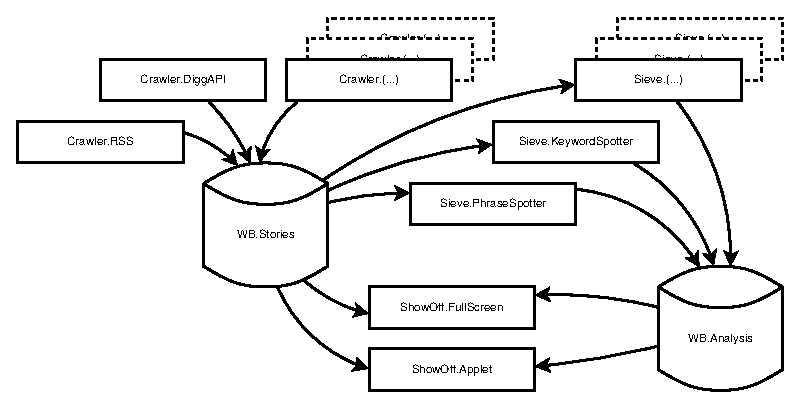
\includegraphics{\designpath/image/global-architecture}
    \caption{\label{fig:global-architecture}Global \Amber\ architecture, the
              names are Psyclone module names}
\end{figure}

\section{\label{sct:modules}Modules}

A complete \Amber\ system will comprise at least three modules running at the
same time; there is a Crawler module, a selector module called Sieve and a
display called ShowOff. The modules are separate executables with their own
life-cycles and resources. Since TCP/IP is used, the executables don't need to
be on the same machine to communicate.

Every module has a specified interface through which communication with
Psyclone is handled.

\subsection{Crawler modules}

When the Crawler is started, it will create one of the available handlers
(depending on what is specified on the command line or what is set as default
during build time). 

It also creates an AirBrush instance to communicate with Psyclone via
Java\-Open\-AIR. The module name announced to Psyclone is `Crawler.' plus the
name of the handler, so `Crawler.RSS' in case of the RSS handler.

After connecting with Psyclone, the handler can get its parameters stored in
the psySpec file and go to work. It will post stories with type `Story'  on the
whiteboard `WB.Stories'.

\subsubsection{RSS}

The RSS crawler module will be fairly straightforward. There are actually quite
a few good RSS parsers around for Java, the only thing the crawler should do is
getting the stories from the RSS feeds along with meta-information and store it
on the whiteboard.

Although the module is called RSS, it can also handle Atom feeds, which is also
quite a popular format.

\begin{module}{Crawler.RSS}
  \trigger{Feed.*}{WB.Control}
  \post{Story}{WB.Stories}
\end{module}

\subsubsection{DiggAPI}

Digg is a website which lets users submit stories found on the web. Other users
then moderate the submissions either by `digging' or `burying' a story. A story
with a lot of `diggs' is a popular one. The nice thing about Digg is that it
actually does a lot of preprocessing work for the \Amber\ system.

Digg
announced\footnote{\url{http://diggtheblog.blogspot.com/2006/07/digg-labs-launches-alpha.html}}
that they will publish a public API within the next months. If time allows, a
DiggAPI module is created.

\begin{module}{Crawler.DiggAPI}
    \post{Story}{WB.Stories}
\end{module}

% \subsubsection{BloggerDataAPI}
% 
% One of the larger weblog hosters is Google with their Blogger service. There
% is an API available to get information from it.
% 
% \begin{module}{Crawler.BloggerDataAPI}
%   \post{Story}{WB.Stories}
% \end{module}


\subsection{Sieve modules}

All analysis modules, or sieves, will get a trigger from a new story on the
whiteboard WB.Stories. They analyse it and if there is anything to say about
the story, a Analysis message is sent to the whiteboard WB.Analyses containing
its judgement on the story.

The contents of this message is specified in Section~\ref{sct:messages}.

Analysis modules may take any time they like to come to a verdict, but it is
possible that a story has already disappeared from the visualization if the
response is very late.

Since all modules employ the same external behaviour, the Psyclone
specification is the same for every one of them.

\begin{module}{Sieve.???}
    \trigger{Story}{WB.Stories}
    \post{Analysis}{WB.Analyses}
\end{module}

\subsection{ShowOff modules}

The ShowOff modules are visualizers which combine the crawled stories from the
Crawler with the analyses from the Sieve modules.

\begin{module}{ShowOff.???}
    \trigger{Story}{WB.Stories}
    \trigger{Analysis}{WB.Analyses}
\end{module}

\subsubsection{Full screen}

The full screen application will display a lot of information and is there to
be looked - not glanced - at. It should be possible to let it do its job
autonomously, just showing a pretty picture, or to be interactive.

\subsubsection{Ambient applet}

The ambient applet will display a very easy to understand image (a glance at it
should be enough) of the status of the page it is on. I.e. if the page is a
weblog, it should display subject information on that weblog, if it is on the
page of a thread of a forum, it displays the flow of the discussion.



\section{\label{sct:messages}Messages}

There are a few message types in the system. Two of which must be defined
system-wide because they are used in the communication between modules.

\subsection{\label{sct:messages:story}Message type `Story'}

The Story message is only posted to the whiteboard `WB.Stories' and only by
Crawler modules.

The message content is a \ac{YAML}\footnote{\url{http://www.yaml.org/}} document
which represents the storyData field inside the Java counterpart of the
message. It contains at least the properties `URI' (to identify the story,
GUIDs are RSS specific and cannot be used), `Author', `Title', `Story-Content'.

It may also contain `Publication-Date' (which is the date of publication in
Internet~Message~Format\cite[Section~3.3]{RFC2822}), `Kind' and other fields.

An example of a YAML document containing Story data:

\begin{verbatim}
---
URI: http://ijsland.luijten.org/2006/09/12/skyr-wasdanou/
Author: Christian Luijten
Title: Skyr... Wasdanou?
Publication-Date: Tue, 12 Sep 2006 21:03:54 +0000
Kind: weblog-posting
Story-Content: >
  Een van die dingen die bij een onbekende cultuur horen zijn de
  eetgewoonten. Elk land heeft zo z’n producten die je nergens
  anders kan krijgen. IJslands nationale zuivelproduct heet Skyr,
  elke oma kan het maken, al is het nogal een hoop werk. Daarom is
  het lange tijd (lees: gedurende de jachtige periode na de tweede
  wereldoorlog toen de Amerikanen hier de boel kwamen ophaasten)
  in ongebruik geraakt, maar op een gegeven moment kwam de vraag
  toch weer terug en zijn een aantal zuivelproducenten het
  industrieel gaan produceren.
\end{verbatim}

\subsection{Message type `Analysis'}

Analysis typed messages are posted on the `WB.Analysis' whiteboard only by
Sieve modules. They contain information about stories present on the
`WB.Stories' whiteboard.

The content of these messages is also YAML format. Stories and Analysis
messages are coupled through their `URI' fields, so this must be present.

An example of a message issued by an analysis module checking for the topic
`Zuivel' (which means dairy products in Dutch):

\begin{verbatim}
---
URI: http://ijsland.luijten.org/2006/09/12/skyr-wasdanou/
Topic: Zuivel
Relation-Strength: 1.0
Author-Strength: 0.1
\end{verbatim}

Its `Relation-Strength' suggests high relevance of the content with the topic.
However, the `Author-Strength' suggests that the author isn't an authority in
the field.

Every analysis module sends a message to the whiteboard if it thinks it is
relevant. It is thus possible that the same URI will get multiple analysis
results or nothing at all, the visualizer module must cope with this and merge
the available information.



% \input{\designpath/04.3-types.inc}



\chapter{Detailed design}

In this chapter, every single class is described in terms of public interface
and functionality. Because of the fairly dynamic character of this project --
new ideas come and go -- this chapter will not be finished until the end of the
project and will probably change regularly.

\section{Files and directories}

All source code will be in the directory \texttt{src/}. All classes are in the
package \texttt{amber} or in a subpackage thereof. The Psyclone specification
file \texttt{psySpec.xml} is found in \texttt{data/}. External libraries that
are redistributed with \Amber\ are in \texttt{lib/}. The source of this
document, the traineeship report and the website are located in
\texttt{documentation/}.

The application is built using Apache
Ant\footnote{\url{http://ant.apache.org/}} and it can be imported into
Eclipse\footnote{\url{http://www.eclipse.org/}}. It requires Java SDK version
1.5 or greater.

\section{Classes}

\begin{figure}[htp]
  \centering
  \includegraphics{image/class-diagram-launcher}
  \caption{The inheritance model of the Launcher class}
  \label{fig:class-diagram-launcher}
\end{figure}

\begin{figure}[p]
  \centering
  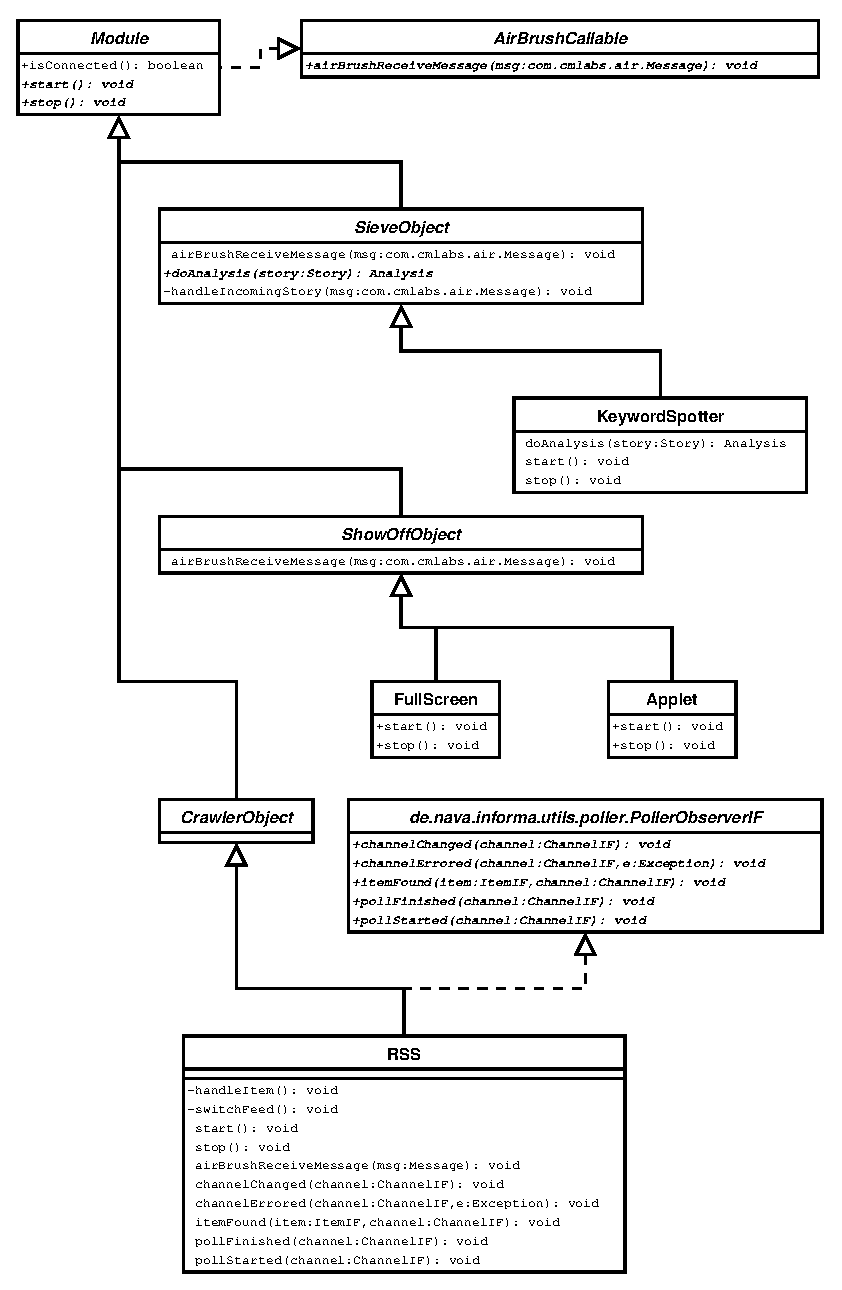
\includegraphics{image/class-diagram-module}
  \caption{The inheritance model of the Module class}
  \label{fig:class-diagram-launcher}
\end{figure}

\begin{figure}[p]
  \centering
  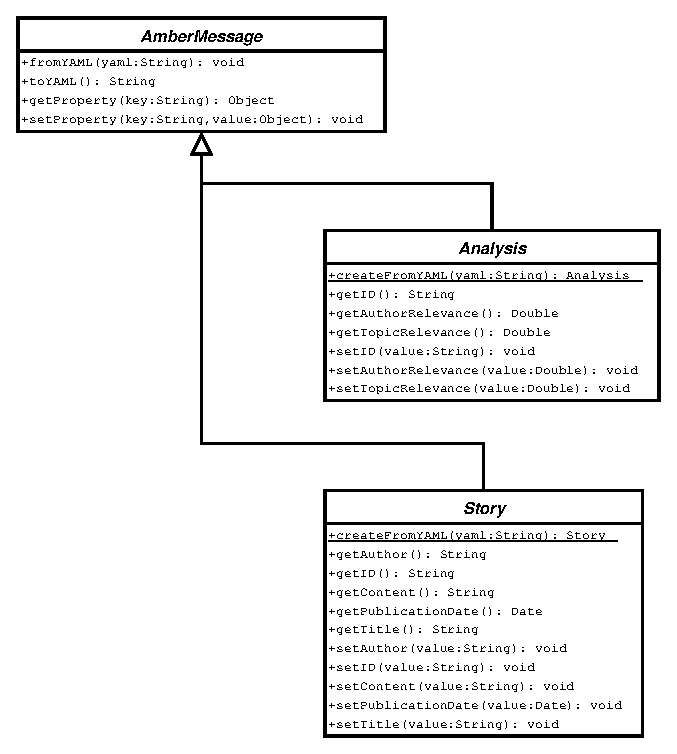
\includegraphics{image/class-diagram-ambermessage}
  \caption{The inheritance model of the AmberMessage class}
  \label{fig:class-diagram-launcher}
\end{figure}

\begin{figure}[p]
  \centering
  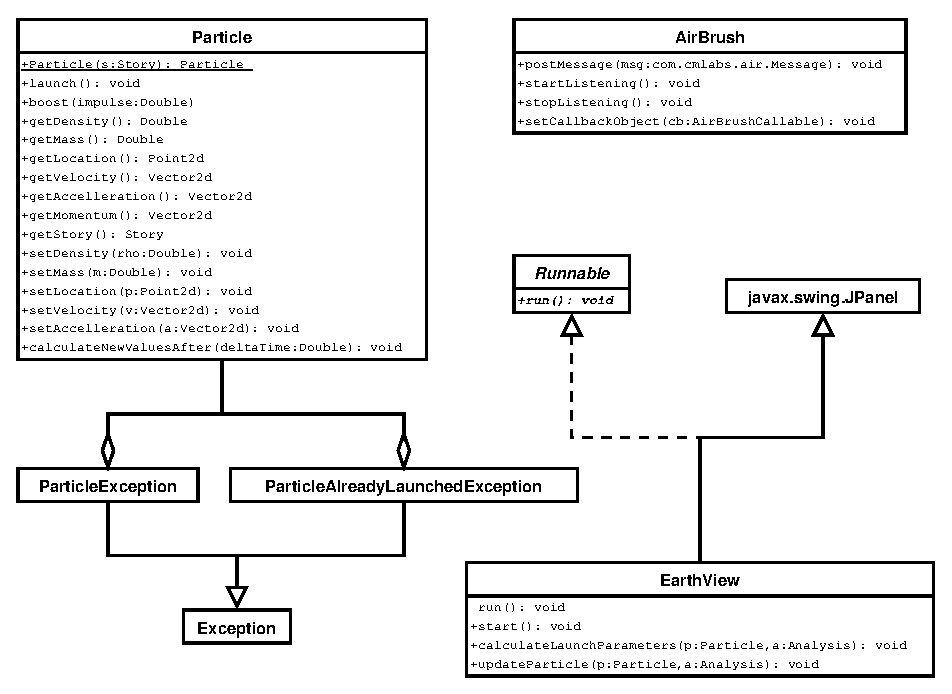
\includegraphics{image/class-diagram}
  \caption{The inheritance model of the remaining classes}
  \label{fig:class-diagram-launcher}
\end{figure}


\section{Objects in the amber package}

The classes in the main package are launchers for the three different modules
and abstract classes for the main objects of these modules. Basically it works
like this; if the Crawler class is started it creates a CrawlerObject and
starts it.

\classname{Crawler}

\begin{classmetadata}
\end{classmetadata}

\begin{interface}
\end{interface}



\classname{CrawlerObject}

\begin{classmetadata}
\end{classmetadata}

\begin{interface}
\end{interface}



\classname{ShowOff}

\begin{classmetadata}
\end{classmetadata}

\begin{interface}
\end{interface}



\classname{ShowOffObject}

\begin{classmetadata}
\end{classmetadata}

\begin{interface}
  \method{\void}{start}{}
    {Starts the ShowOff module.}
  \method{\void}{stop}{}
    {Stops the ShowOff module.}
  \method{\void}{setStoryQueue}{Queue$\langle$Story$\rangle$ q}
    {Sets the queue of incoming stories. ShowOff will handle communication with
    the Psyclone whiteboard and puts stories in the queue.}
\end{interface}



\classname{Sieve}

\begin{classmetadata}
\end{classmetadata}

\begin{interface}
\end{interface}



\classname{SieveObject}

\begin{classmetadata}
\end{classmetadata}

\begin{interface}
\end{interface}



\section{Objects in the amber.common package}

\classname{AirBrush}

\begin{classmetadata}
  \function{Ease communication with Psyclone through JavaOpenAIR.}
\end{classmetadata}

\begin{interface}
  \init{AirBrush}{String moduleName, String hostName, int port}
    {Initializes a connection with Psyclone on \emph{hostName:port} for module
      \emph{moduleName}.}
  \method{\void}{setCallbackObject}{AirBrush\-Callable}
    {Sets the callback object to be used for calls from AirBrush.}
\end{interface}



\interfacename{AirBrushCallable}

\begin{interface}
  \method{\void}{airBrushCallBack}{FIXME}
    {Used as callback function for the AirBrush.}
\end{interface}



\classname{Configuration}

\begin{classmetadata}
\end{classmetadata}

\begin{interface}
\end{interface}



\classname{Object}

\begin{classmetadata}
\end{classmetadata}

\begin{interface}
\end{interface}



\classname{Story}

\begin{classmetadata}
  \function{Storage of Story data.}
  \data{Story has a Map$\langle$String, Object$\rangle$ field where it stores
    all data. It also holds a value with the number of analyses left until it
    is considered enough to be visualized. Instead of thrown back on the
    whiteboard with raw stories, it should then go the the processed stories.}
\end{classmetadata}

\begin{interface}
  \method{\void}{setAuthor}{String}{Sets the author of the story.}
  \method{String}{getAuthor}{}{Gets the author of the story.}
  \method{\void}{setCreationTime}{Date}{Set the creation time of the story}
  \method{Date}{getCreationTime}{}{Get the creation time of the story.}
  \method{\void}{setContent}{String}{Set the content of the story.}
  \method{String}{getContent}{}{Get the content of the story.}
  \method{\void}{setValue}{String k, Object v}
    {Sets an arbitrary object v under keyword k.}
  \method{Object}{getValue}{String k}
    {Gets the object v stored under keyword k.}
  \method{Boolean}{lockForAnalysis}{}
    {Request a lock on the story for analysis. Returns true when given, assumes
      niceness of the analysis modules.}
  \method{\void}{unlock}{}
    {Removes the lock. Again, assumes niceness of the analysis modules.}
  \method{Boolean}{isAnalysisDone}{}
    {Returns true when the story finds it is analysed enough and doesn't need
      another run.}
\end{interface}



\section{Objects in the amber.crawler package}

\classname{Configuration}

\begin{classmetadata}
\end{classmetadata}

\begin{interface}
\end{interface}



\classname{RSS}

\begin{classmetadata}
\end{classmetadata}

\begin{interface}
\end{interface}



\begin{figure}
  \centering
  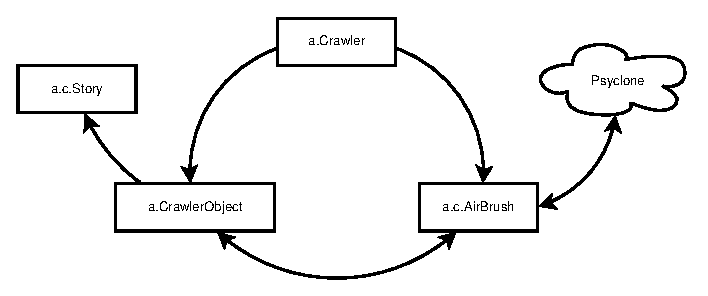
\includegraphics{image/crawler}
  \caption{
    Diagram of the design of the Crawler, the names are Java classnames
  }
\end{figure}



\section{Objects in the amber.sieve package}



\classname{KeywordSpotter}

\begin{classmetadata}
  \extends{SieveObject}
  \implements{amber.common.AirBrushCallable}
  \function{The KeywordSpotter is configured to detect the presence of certain
            keywords in a story which makes it fit in a certain category or
            subject. In early versions the weights of the subjects will be
            equal. In later versions all weights of all subjects of a story
            must for instance add up to 100\%.  This gives the visualizer more
            freedom to place the story.}
\end{classmetadata}

% \begin{interface}
% \end{interface}



\classname{PhraseSpotter}

\begin{classmetadata}
  \extends{SieveObject}
  \implements{amber.common.AirBrushCallable}
  \function{The PhraseSpotter will use a grammar engine to detect whether
            certain types of sentences appear in a story to classify it.}
\end{classmetadata}

% \begin{interface}
% \end{interface}



\subsection{Objects in the amber.showoff package}


\begin{figure}[htp]
  \centering
  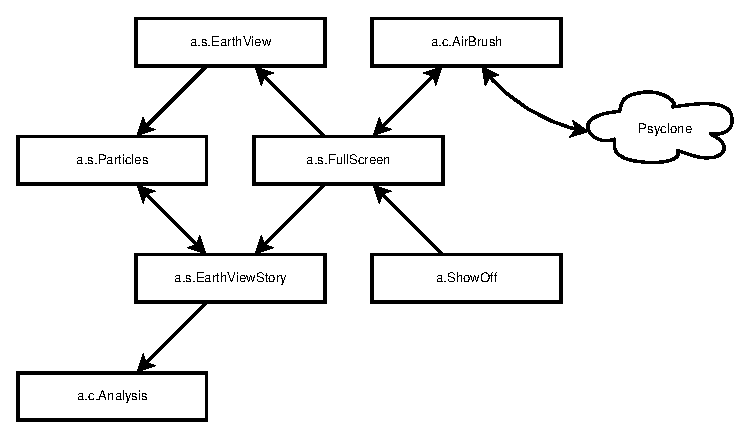
\includegraphics{image/showoff-fullscreen}
  \caption{\label{fig:showoff-fullscreen}Object model of the full screen
    ShowOff module. Arrows represent the presence of references to the object
    where it is pointing to in the object where it is pointing from. The object
    model of the applet is about equal to this one.}
\end{figure}


\classname{Applet}

\begin{classmetadata}
  \extends{amber.ShowOff}
\end{classmetadata}

% \begin{interface}
% \end{interface}


\classname{Attractor}

\begin{classmetadata}
\end{classmetadata}

% \begin{interface}
% \end{interface}


\classname{EarthView}

\begin{classmetadata}
  \extends{javax.swing.JPanel}
  \implements{Runnable}
  \dependencies{FullScreen, StoryLauncher}
  \function{EarthView is a graphical user interface element based on a JPanel
      which displays a picture of Earth in space, with particles orbiting
      around it. Attractors can be added to influence the orbits of the
      particles.}
  \processing{There is a list of particles, which contains information on
      their location and more. EarthView draws each of the particles in the
      list on itself.}
\end{classmetadata}

\begin{interface}
  \init{EarthView}{\mbox{Collection$\langle$Particle$\rangle$} pc}
    {Initializes the EarthView display. It is a child of JPanel and can as such
    be used inside any Swing application. Before starting the Earthview, first
    couple a Particle collection to it using setParticleCollection.}
    \method{\void}{setParticleCollection}{\mbox{Collection$\langle$Particle$\rangle$} pc}
    {Sets the collection of particles to be displayed in the view.}
  \method{\void}{run}{}
    {Runs the thread (for Runnable).}
  \method{\void}{start}{}
    {Starts the thread, lets EarthView draw stuff.}
\end{interface}


\classname{EarthViewStory}


\classname{FullScreen}

\begin{classmetadata}
  \extends{amber.ShowOff}
  \implements{amber.common.AirBrushCallable}
  \dependencies{ShowOff}
  \function{This is a ShowOff module which displays the visualization in full
    screen size.}
\end{classmetadata}

\begin{interface}
  \init{FullScreen}{}
    {Initializes something.}
  \method{\void}{start}{}
    {Start the visualization.}
  \method{void}{airBrushReceiveMessage}{Message msg}
    {}
\end{interface}


\classname{ObservableList}


\classname{Particle}

\begin{classmetadata}
  \function{Storage of particle data.}
  \data{An object of this class has information about its location and
    velocity, and it knows from which story it originates.}
  \dependencies{StoryLauncher, Particles}
\end{classmetadata}

\begin{interface}
  \init{Particle}{Story s}
    {Initializes a particle for Story s.}
  \method{\void}{launch}{}
    {Launches the particle, all parameters must be set, they cannot be changed
      afterwards.}
  \method{\void}{boost}{double}
    {Boost the particle in the direction it is heading. This can happen when
      for instance the Story gets replies or comments; boosting keeps the
      particle around longer.}
  \method{double}{getMass}{}
    {Gets the mass of the particle}
  \method{Point2d}{getLocation}{}
    {Gets the location}
  \method{Vector2d}{getVelocity}{}
    {Gets the velocity}
  \method{Vector2d}{getAcceleration}{}
    {Gets the acceleration}
  \method{\void}{calculate}{double t}
    {Calculates and sets new values using the current values after a period of
      time t}
\end{interface}

The Particles' location is represented by polar coordinates, with ``earth''
being the origin (0, 0).

A particle can be in one of five states: new, launch, orbit, boost or crashed.
Every particle will obviously start in the ``new'' state, after which it is
launched and gets into ``launch'' state. In this state, the $r$ component will
grow until it reaches a set height above the surface of earth, while $\theta$
also accellerates to a set speed. When these values are reached, the particle
will be in orbit and thus in state ``orbit''.

In orbit, a particle slows down and slowly falls back to the earth until it
reaches some lower bound when it is considered ``crashed''. While a particle is
in orbit, it can get a speed increase, it will get in ``boost'' state. During
this period, the height and speed are increased, hereby keeping the particle
orbiting earth for a prolonged time.

While in orbit, a particle can also be attracted by certain attractors that are
located outside the orbits, dependent on the topic of the story it represents.





% \include{\designpath/06-conclusion.inc}

% \appendix

% \chapter{Auto-generated javadoc source code documentation}
% \include{\designpath/design-appendix-javadoc.inc}

\bibliographystyle{cadia}
\bibliography{bibliography}
\addcontentsline{toc}{chapter}{\refname}

\end{document}
